	
\section{Appendix}

\subsection{WSI/D Method in Detail}

\begin{frame}{Proposed Method: Step One}

\begin{itemize}
	\item \textbf{Creation of the linguistic network}
	\begin{itemize}
		\item After preprocessing, we build a HLM $G_{tw}$ that contains the co-occurrent (lexically and syntactically) words for a target word $tw$.
	\end{itemize}

\end{itemize}


\end{frame}

\begin{frame}{Proposed Method: Step Two}
\begin{itemize}

\item \textbf{Computing the similarity between nodes}
	\begin{itemize}
		\item $G_{tw}$ is represented as a bipartite graph $B_{tw}$. Left nodes $U$ represent words and right nodes $W$ correspond to the hyperedges. An edge from a node $u$ to a node $w$ depicts the incidence of node $u$ in hyperedge $w$.
		
		\item A similarity matrix $S_{tw}$ of dimension $|U|\times|U|$ is calculated using the Jaccard similarity: given $n_{i,j} \in U$, then $Jaccard(i,j)=\frac{|N(i)\cap N(j)|}{|N(i)\cup N(j)|}$.
	
		
		\item Induce a new incidence matrix $F_{tw}$ from $S_{tw}$ containing only the closest neighbours to each word $n_i \in U$. Each of these hyperedges represent a set of words that are deemed similar between them according to their Jaccard index value, which must be equal or higher than an assigned threshold $th_1$.
		
	\end{itemize}


\end{itemize}

\end{frame}


\begin{frame}{Proposed Method: Step Three}
\begin{itemize}
	\item \textbf{Clustering words together}
	\begin{itemize}
		\item We select the top $c$-nodes in $F_{tw}$ according to their degree. These nodes are candidate hubs, which must surpass a second threshold $th_2$ to be considered as proper hubs. We use the average Jaccard measure defined for each node $n$ as: $$AvgJaccard(n)=\frac{1}{|hedges(n)|}\sum_{h\in hedges(n)}\frac{\sum_{\substack{i\in h\\j\in h;i\neq j}}Jaccard(i,j)}{|h + 1|}$$ 
		where $hedeges(n)$ is the set of hyperedges $n$ is incident in and its cardinality is defined as $|hedges(n)|$. $|h|$ is the number of nodes in hyperedge $h$. 
		\item Accepted hubs represent senses alongside with their co-occurrent words. The final set of senses is called $SoS_{tw}$.
		
		
		
	\end{itemize}

\end{itemize}
\end{frame}


\begin{frame}{Proposed Method: Step Four}

\begin{itemize}
	\item\textbf{ Word Sense Disambiguation}
	\begin{itemize}
		\item The assignation of a sense consists in looking at each $tw$ instance represented by a context $ct$ and simply determining which sense $s$ in $SoS_{tw}$ shares the highest amount of words with $ct$. The sense $s$ is thus assigned to that instance. 
%		If two senses in $SoS_{tw}$ share the same amount of words with $ct$, one of them is randomly chosen.  This operation is repeated for each instance of each target word. 
	\end{itemize}

\end{itemize}
\end{frame}


\begin{frame}{Experiments}
\begin{itemize}
	\item \textbf{Implementation Framework}
	
	\begin{itemize}
	
		\item \textbf{Systems built and evaluated}: \textbf{DEP} and \textbf{LEX}.
		\begin{itemize}
			\item \textbf{DEP}: Syntactical dependencies
			\item \textbf{LEX}: Lexical co-occurrences 
			
		\end{itemize}
	
		\item \textbf{Two datasets}: Semeval-2007 Task 2 (100 words: 35 nouns, 65 verbs) and Semeval-2010 Task 14 (100 words: 50 nouns, 50 verbs). For brevity, only the results for the first dataset are discussed in this presentation.
		\item \textbf{Evaluation metrics}: Unsupervised evaluation (Paired F-Score, V-Measure). Supervised evaluation (Recall).


	\end{itemize}
	

\end{itemize}
\end{frame}

\begin{frame}{Results Semeval 2010}
\begin{table}[]
\centering

\begin{tabular}{@{}lrrrr@{}}
\toprule
\textbf{VM (\%)} & \textbf{all} & \textbf{nouns} & \textbf{verbs} & \textbf{\#cl} \\ \midrule
{Hermit} & 16.2 & 16.7 & 15.6 & 10.78 \\
NMF$_{lib}$&11.8&13.5&9.4&4.80\\
\textbf{LEX} & 11.6 & 8.8 & 11.9 & 10.5 \\
Random & 4.4 & 4.2 & 4.6 & 4.00 \\
\textbf{DEP} & 3.5 & 3.9 & 2.8 & 2.75 \\
MFS & 0.0 & 0.0 & 0.0 & 1.00 \\ \bottomrule
\end{tabular}
\caption{Unsupervised V-Measure (VM) on the Semeval 2010 test set}
\label{tab:sem2010_VM}
\end{table}


\end{frame}

\begin{frame}{Results Semeval 2010}
\begin{table}[]
\centering

\begin{tabular}{@{}lrrrr@{}}
\toprule
\textbf{FS (\%)} & \textbf{all} & \textbf{nouns} & \textbf{verbs} & \textbf{\#cl} \\ \midrule
MFS & 63.5 & 57.0 & 72.4 & 1.00 \\
Duluth-WSI-SVD-Gap & 63.3 & 57.0 & 72.4 & 1.02 \\
\textbf{DEP} & 53.6 & 50.1 & 58.7 & 2.75 \\
NMF$_{lib}$&45.3&42.2&49.8&5.42\\
\textbf{LEX} & 38.4 & 46.7 & 28.5 & 10.5 \\
Random & 31.9 & 30.4 & 34.1 & 4.00 \\ \bottomrule
\end{tabular}
\caption{Unsupervised Paired F-Score (FS) for the Semeval 2010 test set}
\label{tab:sem2010_FS}
\end{table}
\end{frame}

\begin{frame}{Results Semeval 2010}
\begin{table}
\centering

\begin{tabular}{@{}lrrr@{}}
\toprule
\textbf{SR (\%)} & \textbf{all} & \textbf{nouns} & \textbf{verbs} \\ \midrule
NMF$_{lib}$&62.6&57.3&70.2\\
UoY(2010) & 62.4 & 59.4 & 66.8 \\

\textbf{LEX} & 59.8 & 55.8 & 67.4 \\
\textbf{DEP} & 59.3 & 53.9 & 67.2 \\
MFS & 58.7 & 53.2 & 66.6 \\
Random & 57.3 & 51.5 & 65.7 \\ \bottomrule

\end{tabular}

\caption{Supervised recall (SR) for Semeval 2010 test set (80\% mapping, 20\% evaluation)}
\label{tab:sem2010_SR}
\end{table}
\end{frame}

\subsection{SAEWD}
\begin{frame}{SAEWD: Syntactically Annotated English Wikipedia Dump}

\begin{itemize}
	\item[] \textbf{Building SAEWD}
\end{itemize}

\begin{figure}
\centering
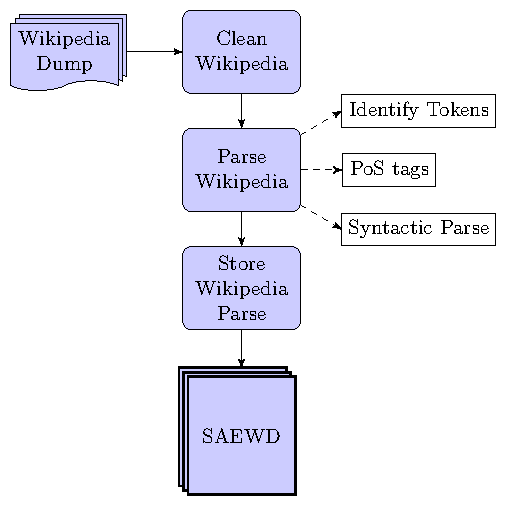
\includegraphics[width=0.5\linewidth]{img/saewd_flow_chart}
\end{figure}

\end{frame}

\begin{frame}{SAEWD: Parsed sample}


			 	\centering	           
	\adjustbox{max height=\dimexpr\textheight-6.5cm\relax,
	           max width=\textwidth}{
\begin{tabular}{llllll}
 \multicolumn{6}{l}{\textit{FILENAME wiki\_00.parsed}}                                           \\ \hline
  \textbf{token}   & \textbf{lemma}   & \textbf{POS} & \textbf{constituency}                      & \textbf{head} & \textbf{dependency} \\ \hline
 \multicolumn{6}{l}{\textit{\%\%\#PAGE Anarchism}}                                         \\ \hline
  {$\vdots$}      &      {$\vdots$}   &  {$\vdots$}   &     {$\vdots$}                              &    {$\vdots$}  &     {$\vdots$}       \\  \hline
 \multicolumn{6}{l}{\textit{\%\%\#SEN 25  9}}                                             \\ \hline
						 A       & a       & DT  & NP\_22,S\_97                      & 3    & det        \\ %\cline{2-7} 
                         great   & great   & JJ  & NP\_22,S\_97                      & 3    & amod       \\ %\cline{2-7} 
                         brigand & brigand & NN  & NP\_22,S\_97                      & 4    & nsubj      \\ %\cline{2-7} 
                         becomes & become  & VBZ & VP\_44,S\_97                      & 0    & root       \\ %\cline{2-7} 
                         a       & a       & DT  & NP\_18,NP\_20,VP\_44,S\_97        & 6    & det        \\ %\cline{2-7} 
                         ruler   & ruler   & NN  & NP\_18,NP\_20,VP\_44,S\_97        & 4    & xcomp      \\ %\cline{2-7} 
                         of      & of      & IN  & PP\_57,NP\_20,VP\_44,S\_97        & 9    & case       \\ %\cline{2-7} 
                         a       & a       & DT  & NP\_18,PP\_57,NP\_20,VP\_44,S\_97 & 9    & det        \\ %\cline{2-7} 
                         Nation  & nation  & NN  & NP\_18,PP\_57,NP\_20,VP\_44,S\_97 & 6    & nmod       \\ %	\cline{2-7} 
\hline 
\end{tabular}}

\end{frame}

\subsection{Ongoing Results}


\begin{frame}{Ongoing Work: Results}
\begin{itemize}
	\item \textbf{Combining the hyperedges: cross fusion}
	
		\item[] Unsupervised paired F-Score (FS) for the Semeval 2007 test set
		\centering
\begin{tabular}{@{}lrrrr@{}}
\toprule
\textbf{FS (\%)} & \textbf{all} & \textbf{nouns} & \textbf{verbs} & \textbf{\#cl} \\ \midrule
1c1word          & 78.9         & 80.7           & 76.8           & 1.00             \\
UBC-AS           & 78.7         & 80.8           & 76.3           & 1.32          \\
\textbf{CROSS$_{k=75}$}     & 78.6         & 80.7           & 76.3           & 1.70          \\
\textbf{DEP}     & 74.9         & 80.2           & 69.0           & 3.27          \\
\textbf{CLUST$_{k=5,th=55	}$}    & 72.5          & 76.0           & 63.8  & 5.47          \\
\textbf{LEX}     & 61.4         & 62.6           & 60.1           & 4.26         \\
UoY(2007)        & 56.1         & 65.8           & 45.1           & 9.28          \\
Random           & 37.9         & 38.1           & 37.7           & 19.7             \\
1c1instance & 	9.5         & 6.6           & 12.7           & 48.51             \\ \bottomrule
\end{tabular}

			
		
\end{itemize}


\end{frame}



